\documentclass{IEEEtran}
\usepackage{graphicx}
\usepackage{hyperref}

\begin{document}

\title{ROBT 310 Image Processing - Project 2 Report}

\author{Anuar Maratkhan}

\maketitle

\section{Introduction}
This is the report for ROBT 310 project 2. The project is aimed to evaluate students' understanding on quantization and intensity transformations that were covered in the previous lectures.

\section{What has been done}
The project consists of three parts: Floyd-Steinberg error diffusion for grayscale image, Floyd-Steinberg error diffusion for colored image (convert to 512 colors image), implementation of additional dithering method where I used dispersed dots (Bayer) method.

\subsection{First part}
For the first part I have used the pseudocode for Floyd-Steinberg error diffusion provided in the project description and function \texttt{find{\_}closest{\_}palette{\_}color} with parameter \texttt{colors} = 2 for binary image with black and white colors. The program starts intensity transformation from the top left element in the matrix (image) and diffuses the image starting from that element. The diffusion matrix used is shown below:

\begin{figure}[h]
	\centering
	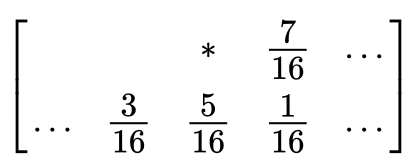
\includegraphics[width=0.2\textwidth]{diffusion_matrix.png}
\end{figure}

The asterisk symbol indicates the current element in the matrix (as like in iteration). Those four elements in 8-adjacency to the current element are diffused then. If those four 8-adjacent elements go out of bound in the image that will cause me an error. Thus, I have used several if statements to fix the error and not go out of image bounds. My \texttt{find{\_}closest{\_}palette{\_}color} method in this case has been choosing either black or white colors corresponding to 0 or 255, respectively. That means if the intensity value is higher than 128 the pixel turns white, otherwise black.

\subsection{Second part}
For the second part I again have used the same pseudocode which I included into a separate function for further usage. But in this part I have been using more colors as was said in the project description, so my \texttt{colors} parameter was equal to 8. For that I have divided the image into three separate matrices corresponding to RGB image channels, and dithered them. Later, I have assigned those dithered matrices to the image. As a result, I got a dithered image.

But for the \texttt{find{\_}closest{\_}palette{\_}color} when I have been using 8 colors in colormap, the function divided my intensity range [0, 255] to 8 parts and assigned the closest color that was in the range of one of those 8 parts. For instance, if I had old pixel intensity was equal to 76 (relatively darker), then the value will be converted to 64 because the value lies in the region between 64 and 96 (value will be floored - round to the closest full integer).

\subsection{Third part}
For the third part I have looked for the methods and how they work a lot. And at the I have chosen the dispersed dots (Bayer) method because it seems to me more efficient (even though there is not that much difference). For understanding how does the Bayer ordered dithering method works I have used \href{https://youtu.be/UJtV3DdjCVY}{this source}. I have chosen the matrix shown below:

\begin{figure}[h]
	\centering
	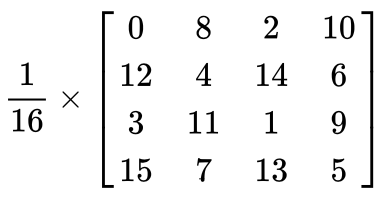
\includegraphics[width=0.2\textwidth]{Bayer_matrix.png}
\end{figure}

The Bayer methods works as follows:

\begin{enumerate}
  \item Multiply the Bayer matrix illustrated above by the number of elements in the matrix;
  \item Add the result of multiplication to the batch of the same size in the image (for that I have used iteration step equal to 4 which indicated the number of rows=cols in Bayer matrix);
  \item Everything that is saturated in the result will be colored as white, otherwise black.
\end{enumerate}

P.S. any threshold map of size length equal to power of two is called \textbf{Bayer matrix}.

P.P.S. I have also considered using \texttt{repmat} function so that I can add only one matrix to the whole image (of the same size so that Bayer matrices will fill the image) but have chosen to do it through iteration.

As a result I got dithered image consisting of black and white dots/intensities:

\begin{figure}[h]
	\centering
	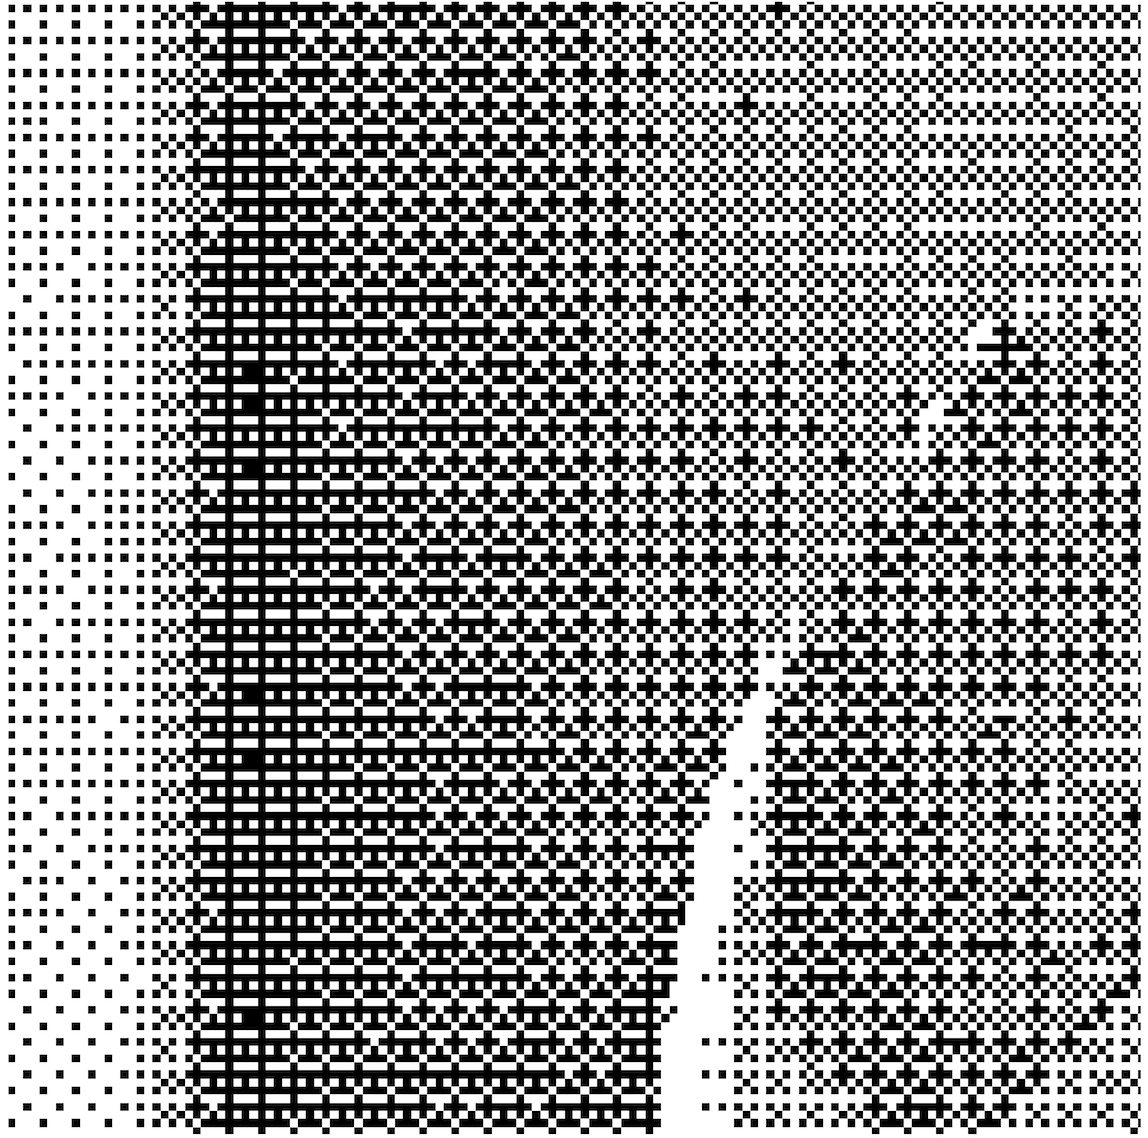
\includegraphics[width=0.20\textwidth]{ordered_result_zoomed.png}
	\caption{Zoomed region of resultant dithered image (Bayer method)}
\end{figure}



\section{How to use it}
The code for the whole project is implemented as a function, which calls other functions, and is named as convention in the project description stated - \texttt{robt310{\_}project2{\_}dither}. So, I have followed the same conventions and to run the function you just need to provide input parameters:

\begin{itemize}
  \item \texttt{input{\_}file{\_}name} - the name of the image of String type which you want to dither
  \item \texttt{output{\_}file{\_}name} - the name of the image of String type where you want to save your result to
  \item \texttt{part} - the number of the part of the project of Integer type (either 1, 2, or 3), where 1 corresponds to the grayscale Floyd-Steinberg error diffusion, 2 corresponds to the colored Floyd-Steinberg error diffusion, and 3 corresponds to grayscale ordered dithering method, otherwise the function will cause an error
\end{itemize}

\section{Additional information}
In fact, I got an easter egg for you (or for myself). I was too curious and implemented the ordered dithering method with Floyd-Steinberg error diffusion at the same time to see how it looks.

Unfortunately, the result stayed the same as ordered dithering and it was not as I expected :(






\end{document}